% REVISÃO DE LITERATURA--------------------------------------------------------

\chapter{HISTÓRICO}
\label{chap:fundamentacaoTeorica}

A Linguagem Python foi concebida no fim dos anos 80, onde sua primeira ideia de implementação surgiu, mais especificamente em 1982, enquanto Guido Van Rossum trabalhava no CWI\footnote{
    O Centrum Wiskunde \& Informatica (Centro de Matemática e Ciência da Computação) é um centro de pesquisa na área de matemática e ciência da computação teórica que faz parte da Organização Holandesa de Pesquisa Científica (NWO).
    Está localizada no Amsterdam Science Park e é conhecido como o local de nascimento de várias linguagens como Algol, Algol 68, NetHack e XHTML.
    Foi membro fundador do Consórcio Europeu de Investigação para Informática e Matemática (ERCIM).
} em Amsterdã, Holanda, no time de desenvolvimento da Linguagem ABC.
Posteriormente, em 1987, com o fim da linguagem ABC, Guido foi transferido para o grupo de trabalho Amoeba — um sistema operacional Microkernel liderado por Andrew Tanenbaum. Foi neste grupo que Guido percebeu a necessidade de uma linguagem para escrever programas intermediários, algo entre o C e o Shell Script.
Tendo como base um código de demonstração da linguagem ABC, alguns elementos de sintaxe e a indentação obrigatória se tornaram grande fonte de inspiração para a nova linguagem.

Em 1989 o desenvolvimento do Python realmente teve início.
Nos primeiros meses de 1990 o autor já possuía uma versão mínima e operacional e, pelo fim do ano de 1990, Python já era mais utilizada no CWI que a própria linguagem ABC.
\par No ano de 1991 Guido foi transferido do grupo Amoeba para o grupo Multimídia.
De acordo com o próprio Guido em uma entrevista com Bill Vennes:
\begin{citacao}
    “ABC me deu a inspiração crucial para Python, o grupo Amoeba a motivação imediata e o grupo de multimídia fomentou seu crescimento".\cite{entrevistaGuido}
\end{citacao}
Ainda neste ano, no dia 20 de Fevereiro, foi lançada a primeira versão do Python, então denominada de \textit{v0.9.0} e anunciada no grupo de discussão alt.sources (\textit{newsgroup})\footnote{
    O alt.sources é um \textit{newsgroup} cujo propósito é ser um repositório de códigos fonte para pessoas que desejam distribuir e compartilhá-los para outras pessoas.
    Não há restrições do tipo, linguagem, máquina ou propósito para o código fonte.\citeonline{alt.sources}
}.
A primeira release era composta de 21 partes que juntos formavam um arquivo $.tar$. 
Nesta primeira versão, o Python já contava com classes, herança, tratamento de exceções, funções, sistema de módulos (empresado da linguagem Modula-3) e os tipos de dado nativos \textit{list, dict, str, e etc}.
\par Desde à primeira versão — e todas as outras versões lançadas dentro do CWI (Python 1.2) — possuíam uma licença derivada da licença MIT.
Abaixo um pequeno histórico de todas as versões lançadas no CWI:
\footnote{A versão 0.9.5 foi disponibilizada apenas para Machintosh}
\begin{table}[!htb]
    \centering
    \caption[Histórico de versão]{Histórico de versão.
    \label{tab:Historico-versao}}
    \begin{tabular}{rrrrr}
        \toprule
        Mês/Ano & versão \\
        \midrule
            Fevereiro de 1991 & 0.9.0  \\
            Fevereiro de 1991 & 0.9.1  \\
            Outubro de 1991 & 0.9.2  \\
            Dezembro de 1991 & 0.9.4  \\
            Janeiro de 1992 & 0.9.5  \\
            Abril de 1992 & 0.9.6  \\
            Janeiro de 1993 & 0.9.8  \\
            Julho de 1993 & 0.9.9  \\
            Janeiro de 1994 & 1.0.0  \\
            Fevereiro de 1994 & 1.0.2  \\
            Maio de 1994 & 1.0.3  \\
            Julho de 1994 & 1.0.4  \\
            Outubro de 1994 & 1.1  \\
            Novembro de 1994 & 1.1.1  \\
            Abril de 1995 & 1.2  \\
        \bottomrule
    \end{tabular}
    \fonte{\citeonline{PyDoc}}
\end{table}

É importante ressaltar que, apesar de a linguagem Python ter sido desenvolvida nas premissas do CWI, este não financiou ou providenciou fundos oficialmente para o desenvolvimento da linguagem.

\section{NOME}

No início de seu projeto, Guido não queria siglas ou um nome fraco, como era o caso da linguagem ABC, ele queria que o nome da linguagem fosse marcante e forte, mas não fazia questão que o nome possuísse um significado profundo.
Guido então decidiu homenagear o grupo britânico de comédia: Monty Python’s Flying Circus, o que se encaixou perfeitamente no “padrão“ de nomear uma linguagem em homenagem a pessoas famosas\footnote{
    Vide: Pascal, Ada, Eiffel.
} e à tradição do CWI de utilizar nomes de programas de TVs para projetos.
 
Por anos o autor evitou vincular a linguagem ao réptil (a cobra píton) mas desistiu quando a editora O’Reilly — que possui a tradição de utilizar animais nas capas de seus livros — sugeriu colocar uma cobra píton na capa do seu primeiro livro "Programming Python".
\begin{figure}[!htb]
    \centering
    \caption{Mount Python’s Logo}
    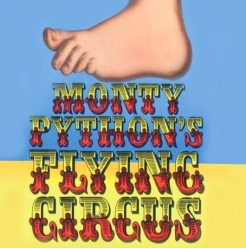
\includegraphics[width=0.5\textwidth]{./dados/figuras/mount-python.png}
    \fonte{\citeonline{MountPython}}
    \label{fig:figura-mountPython}
\end{figure}

\section{COMUNIDADE}

A primeira “comunidade” do Python surgiu formalmente com a criação do \textit{newsgroup: comp.lang.python na Usenet}, em março de 1993.
Posteriormente, este \textit{newsgroup} foi migrado para uma lista de discussão por e-mail, tendo como base o \textit{GNU Mailman}, um gerenciador de listas software livre escrito em Python.
\par No verão de 1994, o grupo iniciou uma discussão intitulada “Se Guido fosse atingido por um ônibus?”\footnote{
    \citeonline[p. ~1]{bus}
}.
Por mais mórbido que essa discussão soava, ela tocava no âmago da comunidade Python, pois Guido era seu principal desenvolvedor e ele tomava as decisões, criando assim o medo do Python desaparecer com seu criador.
Muitos justificavam que a política de “um homem só” reduziam as possibilidades de doação e investimento na linguagem.
Visto isso, nesta discussão, nasceu a necessidade de se criar um padrão ou organização responsável pelo Python, desvinculando Guido como o único responsável (e detentor de seus direitos) e garantindo assim a existência prolongada da linguagem.
 
No início de 2000, Guido, Barry Warsaw, Jeremy Hylton e Fred Drake receberam o convite para ser juntar à \textit{startup} BeOpen.com, uma iniciativa que estava recrutando diversos desenvolvedores \textit{Open Source}.
Antes de deixar a CNRI\footnote{
    A Corporation for National Research Initiatives (CNRI) é uma organização sem fins lucrativos formada em 1986 localizada em Virginia, Estados Unidos.
    Com o objetivo de empreender, fomentar e promover pesquisas de interesse público, as atividades giram em torno do desenvolvimento estratégico de tecnologias de informação baseadas em rede.
    A instituição fornece liderança e financiamento para pesquisa e desenvolvimento de infraestrutura de informação.\citeonline{cnri}
} os desenvolvedores foram forçados a lançar a versão 1.6, para finalizar o ciclo de desenvolvimento do Python.

Para a versão 1.6 a CNRI insistiu em utilizar uma licença escrita pelos seus próprios advogados.
Como esperado, esta licença diferia da utilizada até o momento, visando controlar “os direitos do Python” e submetendo o software às leis do estado da Virginia.
Como o Python era utilizado pelo GNU Mailman, a FSF (Free Software Foundation) estava receosa que essa nova licença pudesse restringir o uso de ambos os softwares. 
Desta forma, Richard Stallman e Eben Moglen (ambos da PSF\footnote{
    Vide: página \pageref{sec:python-software-foundation}, secção: \textit{Python Software Foundation}
}), analisaram a licença e chegaram a conclusão de que esta não era uma licença compatível com as premissas do software livre.
Com o apoio de Eric Raymond e da PSF a licença foi reescrita para satisfazer tanto a FSF quanto a CNRI.
A versão 1.6 foi lançada em Setembro de 2000, sendo que o grupo de desenvolvedores já estavam na BeOpen.com desde Maio de 2000.
\begin{figure}[!htb]
    \centering
    \caption{Free Software Foundation's Logo}
    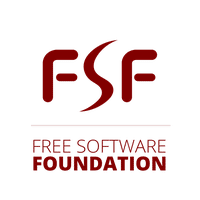
\includegraphics[width=0.5\textwidth]{./dados/figuras/FSF.png}
    \fonte{\citeonline{FSF}}
    \label{fig:figura-fsf}
\end{figure}

Devido a esta história do Python, a licença do Python era vista “em camadas”.
Na base tínhamos a licença do CWI, seguida pela licença do CNRI (no meio) e por último a licença da BeOpen.com.
Apesar da confusão, a licença era compatível com o modelo OSI que define uma licença Open Source e também é compatível com a GNU GPL (General Public License), garantindo as liberdades de um software livre.

\section{\textit{BeOpen.com} \& \textit{Digital Creations}}
Ja na BeOpen.com foi formado o grupo PythonLabs e a versão 2.0 do Python foi lançada em outubro de 2000.
O Python 2.0\footnote{
    A estadia na BeOpen.com rendeu apenas uma release do Python, a versão 2.0 citada anteriormente, pois em Outubro de 2000 ocorreu a falência e desmembramento da BeOpen.com e o PythonLabs foi contratado pela empresa Digital Creations.
} utilizava uma versão alterada da licença presente na versão 1.6 (alterando apenas o responsável para BeOpen.com).
Nesta estadia o Python (como comunidade e linguagem) evoluiu significativamente:
\begin{itemize}
    \item Os desenvolvedores passaram a se focar exclusivamente para o Python
    \item O desenvolvimento foi centralizado, utilizando um servidor CVS no SourceForge
    \item Por volta de 30 pessoas possuíam acesso de commit
    \item Banco de dados de patches e bugs também eram hospedados no SourceForge
    \item Criação das PEPs (Python Enhancement Proposal)
\end{itemize}

\begin{figure}[!htb]
    \centering
    \caption{Zope Logo}
    
\includegraphics[width=0.5\textwidth]{./dados/figuras/zope.png}
    \fonte{\citeonline{zope}}
    \label{fig:figura-zope}
\end{figure}

Em paralelo à esta contratação [\textit{Digital Creations}], o PythonLabs recebeu também convites de outras duas empresas, a VA Linux e a ActiveState.
Posteriormente a Digital Criations mudou de nome e ficou conhecida como Zope Corporation, referência ao seu produto mais conhecido, o Web CMS (Content Managing System) Zope.
Parte da mudança para da Zope Corporaton foi influenciada pela certeza de que o futuro do Python não podia ser influenciado pelos objetivos e ideais daqueles para os quais Guido trabalhava.
Foi então que criaram a Python Software Foundation (PSF).

\section{\textit{Python Software Foundation}}
\label{sec:python-software-foundation}
Python Software Foundation
Em 2001 foi criada a Python Software Foundation (PSF), uma organização sem fins lucrativos constituída por membros da equipe de desenvolvimento (daquela época) e por Eric Raymond.
Ela tem como objetivo ser dona de qualquer propriedade intelectual relacionada ao Python, e como missão promover e proteger o avanço da linguagem Python, além suportar e auxiliar o crescimento de comunidades de programadores Python.
Ela possui diversos patrocinadores como:
\begin{itemize}
    \item ActiveState;
    \item Advanced Simulation Technology Inc. (ASTi);
    \item Array BioPharma, Inc.;
    \item BizRate.com;
    \item Canonical;
    \item Globo;
    \item Google;
    \item Lucasfilm;
    \item Microsoft;
    \item OpenEye Scientific Software;
    \item O’Reilly Media, Inc.;
    \item Red Hat;


\end{itemize}
 
 
Em dezembro de 2008 é lançada a versão 3 do Python, mas ainda manteve muitos adeptos na versão 2, tanto que ambas são retrocompatíveis apesar da 2ª não ser mais recomendada para novos projetos.
 
 
Após a criação da PSF todas as \textit{releases} desde a 2.1 foram feitas utilizando a PSF License Agreement, uma licença que atribui todos os direitos do Python à PSF.
A licença está disponível na íntegra na documentação oficial do Python.
Uma vez que o futuro do Python (e a sua evolução) se desvinculou dos empregadores de seu criado, existem poucos relatos e registros.
Segue alguns destaques:
\begin{itemize} 
    \item Em Julho de 2003 o PythonLab saiu da Zope Corporation para trabalhar na Elemental Security em San Mateo, California;
    \item Em Dezembro de 2005 Guido foi trabalhar no Google em Mountain View, Califórnia;
    \item Em Janeiro de 2013 Guido foi trabalhar para o Dropbox.
\end{itemize}
